% Provenance (never printed): see sources/outline_sources.md (Year 3: the
% Rayleigh number; thermal boundary layers; slab pull and ridge push; plumes;
% post-glacial rebound and mantle viscosity). Brief: sources/book5/BRIEFS.md,
% ch. 6. Curves from figdata/bachelor-3/convection_scaling.py (PREM read only),
% gia_relaxation.py and ridge_push.py (on plate_cooling.py). Exercise and
% problem values in the Book 5 scratch calculator calc/ch06.py.
\chapter{الحمل في الوشاح والقوى المحرّكة للصفائح}\label{ch:b3:mantle-convection}

يرتفع ساحل شمال السويد من البحر بنحو سنتيمتر واحد في
السنة، بعد عشرة آلاف سنة من ذوبان الغطاء الجليدي الذي كان يغطيه؛
وترتفع سواحل خليج هدسون بالسرعة نفسها. لا يدفعها إلى أعلى سوى الوشاح،
يتدفّق ببطء عائدًا أسفل الموضع الذي ضغطه الجليد نحو الأسفل. ويدلّ معدّل
ارتداد الأرض على \omterm{def:b3:mantle-convection:gia}{لزوجة الوشاح}، وتحدّد اللزوجة نفسها
سرعة حمل الوشاح وحركة الصفائح. يتساءل هذا الفصل
لماذا يحمل الوشاح الصلب أصلًا، وبأيّ سرعة يجب أن يتدفّق لينقل
حرارة الأرض، وما القوى التي تحرّك الصفائح، وماذا يقول ارتداد
الأرض عن \omterm{def:b3:mantle-convection:gia}{لزوجة الوشاح}.
% ledger: vestol19:umea, zhao12:fenno, sella07:gia

\begin{recall}
اللزوجة، أي الجريان الزاحف لمائع لزج (معادلات ستوكس
$\nabla p = \eta\nabla^2\mathbf u$، $\nabla\cdot\mathbf u = 0$)، وقانون ستوكس
للكرة، وعدد رينولدز والطفو واردة في
المجلّدات الجامعية لكتب الفيزياء. وقد ورد الحمل في الوشاح والارتداد
الأيزوستاتي في مجلّد المرحلة الثانوية (الصف 12)، \omterm{prop:b3:mantle-convection:ridge-push}{وقوة دفع الظهرة} وشدّ اللوح المندس في جزئه الخاص بالصف 11.
الطبقة الحدّية الحرارية والغلاف الصخري الحراري والمنحنى الأدياباتي للوشاح
موجودة في مجلد السنة الأولى، في فصلها عن ميزانية الحرارة الأرضية؛ والبقع الساخنة،
وأعمدة الوشاح والأقاليم البركانية الكبرى في فصلها عن البقع الساخنة.
ويرد \omterm{def:b3:lithosphere-thermal-models:half-space}{نموذج تبريد نصف الفضاء} في \cref{ch:b3:lithosphere-thermal-models}،
\omterm{def:b3:gravity-geodesy:flexure}{وانثناء الغلاف الصخري} في \cref{ch:b3:gravity-geodesy}،
\omterm{def:b3:seismology-imaging:tomography}{والتصوير المقطعي الزلزالي} في \cref{ch:b3:seismology-imaging}.
\end{recall}

\section{لماذا يحدث الحمل في الوشاح}

الوشاح صلب، إذ ينقل الموجة S. غير أنّه على مدى ملايين السنين
يزحف زحفًا كمائع بالغ اللزوجة، وطبقةٌ من مائع تُسخَّن من
الأسفل وتُبرَّد من الأعلى قد تبقى ساكنة، وتعبرها الحرارة
بالتوصيل، أو تنقلب. كتلةٌ من مائع ساخن حجمها $d$، أخفّ من
محيطها بمقدار $\rho\alpha\,\Delta T$، ترتفع بسرعة من رتبة
$\rho g\alpha\,\Delta T d^2/\eta$؛ وتفقد حرارتها بالانتشار خلال زمن من
رتبة $d^2/\kappa$. فإن استطاعت أن ترتفع عبر الطبقة قبل أن تبرد،
تنقلب الطبقة.

\begin{definition}[عدد رايلي]\label{def:b3:mantle-convection:rayleigh}
بالنسبة لطبقة مائعة سُمكها $d$، وكثافتها $\rho$، ومعامل التمدّد الحراري
$\alpha$، والانتشارية الحرارية $\kappa$ واللزوجة $\eta$، تحت تأثير
الجاذبية $g$، وبفرق درجة الحرارة $\Delta T$ بين قاعدتها
وقمّتها، فإنّ \emph{عدد رايلي}\index{عدد رايلي} هو
\[
  \mathrm{Ra} = \frac{\rho g\alpha\,\Delta T d^3}{\kappa\eta},
\]
أي نسبة زمن الانتشار $d^2/\kappa$ إلى زمن الارتفاع بالطفو
$\eta/(\rho g\alpha\,\Delta Td)$.
\end{definition}

\begin{definition}[عدد رايلي الحرج]\label{def:b3:mantle-convection:critical}
\emph{عدد رايلي الحرج}\index{عدد رايلي الحرج}
$\mathrm{Ra}_c$ لطبقة ما هي قيمة \omterm{def:b3:mantle-convection:rayleigh}{عدد رايلي} التي فوقها
يكبر الاضطراب الصغير في حالة السكون فيتحوّل إلى حمل، وأدنى منها
يتلاشى.
\end{definition}

\begin{proposition}[بداية الحمل]\label{prop:b3:mantle-convection:onset}
لطبقة خلا سطحاها العلوي والسفلي من إجهاد القصّ، وثُبِّتت درجتا حرارتهما
ثابتتين، ينمو اضطراب ذو عدد موجي أفقي $k$ (بوحدات $1/d$)
عندما $\mathrm{Ra} > (\pi^2 + k^2)^3/k^2$. وتبلغ أدنى قيمة للطرف الأيمن،
عند $k = \pi/\sqrt2$، ما يعطي
\[
  \mathrm{Ra}_c = \frac{27\pi^4}{4} \approx 657.5,
\]
وأولى الخلايا التي تظهر بعرض $2\sqrt2\,d$. وبين حدود صلبة،
$\mathrm{Ra}_c \approx 1708$.
\end{proposition}

\admitted
تحليل الاستقرار الخطّي الذي يقوم عليه، وهو اضطراب لمعادلتي الحرارة وستوكس
حول الحالة التوصيلية، وهو وارد في معالجة كتب الفيزياء
للحمل؛ ويتحقّق التمرين 11 من الحدّ الأدنى.

يُظهر الشكل أدناه الطبقة التي يحدث فيها الحمل. وقيم الوشاح، مع
عمق الحدّ بين اللبّ والوشاح، $d = \qty{2891}{km}$، والكثافة المتوسطة للوشاح،
\qty{4476}{kg.m^{-3}}، و$g$ بين 9.8
و\qty{10.7}{m.s^{-2}}، وكلّها مأخوذة من نموذج الأرض الزلزالي PREM؛ و$\alpha =
\qty{3.1e-5}{K^{-1}}$ و$\Delta T = \qty{1450}{K}$ من نموذج الصفيحة في
\cref{ch:b3:lithosphere-thermal-models}؛ و$\kappa = \qty{e-6}{m^2.s^{-1}}$؛
و$\eta$ بين \num{e21} و\qty{e22}{Pa.s} (انظر \cref{sec:b3:mantle-convection:gia})،
فتعطي $\mathrm{Ra}$ بين \num{4.9e6} و\num{4.9e7}، نحو سبعة آلاف إلى
سبعين ألف مرّة قيمة الحدّ الحرج. فلا يستطيع الوشاح إلّا أن يحمل.
% ledger: data:prem, honda04:gdh1, delaney86:properties, mitrovica96:haskell, milne04:bifrost

\begin{omfigure}
\begin{tikzpicture}[font=\scriptsize, x=1cm, y=1cm]
\fill[blue!10] (0,3.4) rectangle (10,3.0);
\fill[red!12] (0,0) rectangle (10,0.4);
\draw[thick] (0,0) rectangle (10,3.4);
\node[above] at (5,3.4) {\foreignlanguage{arabic}{القمّة الباردة، $T_0$}};
\node[below] at (5,0) {\foreignlanguage{arabic}{القاعدة الساخنة، $T_0 + \Delta T$}};
\foreach \c/\s in {1.25/1, 3.75/-1, 6.25/1, 8.75/-1} {
  \draw[gray!70!black, thick] (\c,1.7) ellipse[x radius=0.95, y radius=1.05];
  \draw[->, gray!70!black, thick] ({\c+0.25*\s},2.75) -- ({\c-0.3*\s},2.75);
  \draw[->, gray!70!black, thick] ({\c-0.25*\s},0.65) -- ({\c+0.3*\s},0.65);
}
\draw[->, red!70!black, very thick] (2.5,0.45) -- (2.5,2.9);
\draw[->, red!70!black, very thick] (7.5,0.45) -- (7.5,2.9);
\draw[->, blue!70!black, very thick] (5,2.95) -- (5,0.5);
\node[red!70!black, fill=white, inner sep=1pt, align=center] at (2.5,1.7) {حارّ\\صعود};
\node[red!70!black, fill=white, inner sep=1pt, align=center] at (7.5,1.7) {حارّ\\صعود};
\node[blue!70!black, fill=white, inner sep=1pt, align=center] at (5,1.7) {بارد\\هبوط};
\draw[<->] (10.3,0) -- (10.3,3.4) node[midway, right] {$d$};
\draw[<->] (-0.25,3.0) -- (-0.25,3.4) node[midway, left] {$\delta$};
\draw[<->] (-0.25,0) -- (-0.25,0.4) node[midway, left] {$\delta$};
\node[anchor=west] at (10.6,3.2) {الطبقة الحدّية العليا};
\node[anchor=west] at (10.6,0.2) {الطبقة الحدّية السفلى};
\end{tikzpicture}

\par\smallskip{\small الحمل في طبقة تُسخَّن من الأسفل وتُبرَّد من
أعلى. تعبر الحرارة الطبقات الحدّية الرقيقة، ذات السماكة $\delta$، بالتوصيل؛
في ما بينهما يحمل الداخل جيّد الخلط الحرارة بالجريان. تنفصل صفائح باردة
عن الطبقة العليا وتغوص؛ وتصعد صفائح حارّة من
السفلى.}\label{fig:b3:mantle-convection:cell}
\end{omfigure}

ويُسخَّن الوشاح كذلك من داخله، بتحلّل العناصر المشعّة،
ومن الأسفل، بفعل اللبّ. الطبقة المُسخَّنة من داخلها وحدها لا تملك
طبقة حدّية حارّة عند قاعدتها: يُدفع جريانها بصفائح باردة تهبط من
الأعلى، بينما يكون الجريان الصاعد عودةً واسعةً سلبية. والألواح المندسة من هذه الصفائح،
والأعمدة تحتاج إلى الحرارة القادمة من اللبّ.

\section{الطبقات الحدّية وقوّة الحمل}

\begin{definition}[عدد نوسلت]\label{def:b3:mantle-convection:nusselt}
يُعرَّف \emph{عدد نوسلت}\index{عدد نوسلت} لطبقة يجري فيها الحمل بأنّه
نسبة التدفق الحراري عبرها إلى التدفق الذي يحمله التوصيل وحده
عبر الطبقة نفسها، $\mathrm{Nu} = q\,d/(k\,\Delta T)$.
\end{definition}

\begin{theorem}[قياس الحمل بالطبقة الحدّية]\label{thm:b3:mantle-convection:scaling}
في طبقة يجري فيها الحمل عند $\mathrm{Ra} \gg \mathrm{Ra}_c$، إذا نمت كلّ طبقة حدّية حرارية
حتى يبلغ \omterm{def:b3:mantle-convection:rayleigh}{عدد رايلي} الخاص بها، المبنيّ على سماكتها
$\delta$ وفرق درجة الحرارة $\Delta T/2$ عبرها، يبلغ
$\mathrm{Ra}_c$، فإنّ
\[
  \delta = d\Bigl(\frac{2\mathrm{Ra}_c}{\mathrm{Ra}}\Bigr)^{1/3},\qquad
  \mathrm{Nu} = \frac12\Bigl(\frac{\mathrm{Ra}}{2\mathrm{Ra}_c}\Bigr)^{1/3},
  \qquad
  u = \frac\kappa d\Bigl(\frac{\mathrm{Ra}}{2\mathrm{Ra}_c}\Bigr)^{2/3},
\]
حيث $u$ هو مقياس سرعة الجريان، المعرَّف باشتراط أن
تنمو الطبقة إلى $\delta$ بينما يعبر المائع الخليّة. وهذا هو
\emph{قياس الحمل بالطبقة الحدّية}\index{قياس الحمل بالطبقة الحدّية}.
\end{theorem}

\begin{proof}
يكون الداخل جيّد الخلط عند متوسط درجة الحرارة، فتحمل كلّ طبقة حدّية
نصف $\Delta T$. \omterm{def:b3:mantle-convection:rayleigh}{وعدد رايلي} لها هو $\rho g\alpha(\Delta T/2)
\delta^3/(\kappa\eta) = \mathrm{Ra}\,(\delta/d)^3/2$؛ وبجعله مساويًا
$\mathrm{Ra}_c$ فنحصل على $\delta$. ويُوصَّل التدفق الحراري عبر الطبقة،
$q = k(\Delta T/2)/\delta$، فيكون $\mathrm{Nu} = qd/(k\Delta T) = d/(2\delta)$.
تنمو طبقة حدّية بالانتشار حتى السماكة $\delta$ خلال زمن
$\delta^2/\kappa$؛ ويعبر المائع عند القمة الخليّة، التي عرضها من رتبة
$d$، في زمن $d/u$. وبمساواة الزمنين، $u = \kappa d/\delta^2 =
(\kappa/d)(d/\delta)^2$.
\end{proof}

لا يزداد التدفق الحراري إلّا بمقدار الجذر التكعيبي للعدد $\mathrm{Ra}$:
فلزوجة أدنى بمائة مرّة تُعطي حرارة أكثر بأقلّ من خمس مرّات.
ومع \omterm{def:b3:mantle-convection:rayleigh}{عدد رايلي} للوشاح $\mathrm{Ra} = \num{4.9e7}$، يُعطي القياس $\delta \approx \qty{87}{km}$،
$\mathrm{Nu} \approx 17$، وتدفّقًا حراريًا قدره $\mathrm{Nu}\,k\Delta T/d \approx
\qty{26}{mW.m^{-2}}$ مع $k = \qty{3.1}{W.m^{-1}.K^{-1}}$، و$u \approx
\qty{1.2}{cm/yr}$ (الشكل أدناه). وتساوي الطبقة الحدّية سماكة الصفيحة المحيطية في
\cref{ch:b3:lithosphere-thermal-models}، \qty{95}{km}؛ أمّا
الجذر التربيعي المتوسّط لسرعات الصفائح اليوم، فيتراوح من \qty{1.1}{cm/yr} (أمريكا الجنوبية)
إلى \qty{7.5}{cm/yr} (كوكوس)، و\qty{4.4}{cm/yr} للغلاف
الصخري كلّه. ويبلغ متوسط التدفق الحراري للأرض \qty{92}{mW.m^{-2}}،
ثلاثة إلى أربعة أضعاف القياس: فالحرارة المتولّدة داخل الوشاح، التي تُغفلها طبقة
مُسخَّنة من الأسفل، والثوابت من رتبة الواحد التي يُغفلها القياس
كلاهما يسهم في الفرق. وأمّا قانون بمدخل واحد، فرتب المقادير
صحيحة: فالصفائح هي الطبقة الحدّية العليا لوشاح ذي $\mathrm{Ra}
\sim 10^7$.
% ledger: nnr56:rms, b2dd10:continents, honda04:gdh1

\begin{omfigure}
\begin{tikzpicture}
\begin{groupplot}[group style={group size=1 by 2, vertical sep=2.5cm},
  omrecord, width=0.86\linewidth, height=0.40\linewidth, xmode=log, ymode=log,
  xmin=100, xmax=1e10, xlabel={عدد رايلي $\mathrm{Ra}$}]
\nextgroupplot[ylabel={عدد نوسلت}, ymin=0.3, ymax=300,
  title={(أ) التدفق الحراري بوحدات تدفق التوصيل}, title style={font=\small}]
% computed in figdata/bachelor-3/convection_scaling.py; ledger: data:prem, honda04:gdh1
\addplot[omDef, thick] table[x=ra, y=nu] {figdata/out/bachelor-3-convection_scaling-conduction.dat};
\addplot[red!70!black, thick] table[x=ra, y=nu] {figdata/out/bachelor-3-convection_scaling-scaling.dat};
\addplot[gray, densely dashed, unbounded coords=jump] table[x=ra, y=y] {figdata/out/bachelor-3-convection_scaling-band.dat};
\draw[gray, densely dotted] (axis cs:657.5,0.3) -- (axis cs:657.5,1);
\node[font=\scriptsize, anchor=west] at (axis cs:700,0.45) {$\mathrm{Ra}_c$};
\node[font=\scriptsize, anchor=south west, omDef] at (axis cs:115,1.08) {التوصيل};
\node[font=\scriptsize, anchor=north west, red!70!black] at (axis cs:3e4,0.95) {$\tfrac12(\mathrm{Ra}/2\mathrm{Ra}_c)^{1/3}$};
\node[font=\scriptsize, fill=white, inner sep=1pt] at (axis cs:1.55e7,120) {الوشاح};
\nextgroupplot[ylabel={السرعة \babelsublr{(\unit{cm/yr})}}, ymin=1e-3, ymax=100,
  title={(ب) مقياس السرعة عند $d = \qty{2891}{km}$}, title style={font=\small}]
\addplot[red!70!black, thick] table[x=ra, y=u] {figdata/out/bachelor-3-convection_scaling-scaling.dat};
\addplot[gray, densely dashed, unbounded coords=jump] table[x=ra, y=y] {figdata/out/bachelor-3-convection_scaling-band.dat};
\addplot[blue!70, thick, dash dot, unbounded coords=jump] table[x=ra, y=u] {figdata/out/bachelor-3-convection_scaling-plates.dat};
\node[font=\scriptsize, anchor=south west, blue!60!black] at (axis cs:150,7.6) {أسرع صفيحة};
\node[font=\scriptsize, anchor=north west, blue!60!black] at (axis cs:150,1.0) {أبطأ صفيحة};
\node[font=\scriptsize, fill=white, inner sep=1pt] at (axis cs:1.55e7,0.004) {الوشاح};
\end{groupplot}
\end{tikzpicture}

\par\smallskip{\small قياس الحمل. (أ) دون $\mathrm{Ra}_c$ تنقل الطبقة الحرارة
بالتوصيل ($\mathrm{Nu} = 1$)؛ وأعلى منه بكثير، فيُرسم قانون الطبقة الحدّية،
من $\mathrm{Ra} = 16\,\mathrm{Ra}_c \approx \num{1.1e4}$، حيث يُعطي $\mathrm{Nu} = 1$ (وبين الحالتين
يبدأ الحمل تدريجيًا). (ب) مقياس السرعة
لعمق الوشاح و$\kappa = \qty{e-6}{m^2.s^{-1}}$، مع
مدى سرعات الصفائح اليوم (بخطّ شرطي-نقطي). وتحدّ الخطوط المتقطّعة \omterm{def:b3:mantle-convection:rayleigh}{عدد رايلي} للوشاح
عند لزوجتين \num{e22} و\qty{e21}{Pa.s}.}\label{fig:b3:mantle-convection:scaling}
\end{omfigure}

\section{القوى المؤثّرة في الصفيحة}

تتحرّك الصفيحة بسرعة ثابتة، فتتوازن القوى المؤثّرة فيها. وتدفعها ثلاث قوى أو تقاومها
من حوافّها وقاعدتها (الشكل أدناه). والقوّة التي يؤثّر بها اللوح المندس الغائص في صفيحته،
أي شدّ اللوح المندس، تنشأ عن الكثافة الزائدة للوح مندس بارد في الوشاح الأدفأ.
أمّا قوّة دفع الظهرة، وهي دفع الظهرة المرتفعة الساخنة للصفيحة الأبرد المجاورة لها، فتُستنتج من
\omterm{def:b3:lithosphere-thermal-models:half-space}{نموذج تبريد نصف الفضاء} في
\cref{ch:b3:lithosphere-thermal-models}.

\begin{omfigure}
\begin{tikzpicture}[font=\scriptsize, x=1cm, y=1cm]
\fill[orange!12] (0,-0.6) rectangle (12.6,-6.0);
\fill[blue!8] (0,0) -- (0,-0.6) .. controls (3,-1.0) and (6,-1.25) .. (8.4,-1.3) -- (8.9,-1.9) -- (10.6,-0.2) -- (10.6,0) -- cycle;
\fill[gray!35] (0,-0.6) .. controls (3,-1.0) and (6,-1.25) .. (8.4,-1.3) -- (8.9,-1.9) -- (11.2,-5.0) -- (10.3,-5.6) -- (8.4,-2.9) .. controls (6,-2.85) and (3,-2.4) .. (0.2,-0.95) -- cycle;
\fill[gray!18] (10.6,-0.2) -- (12.6,0.1) -- (12.6,-2.5) -- (11.7,-2.5) -- (8.9,-1.9) -- cycle;
\draw[thick] (0,-0.6) .. controls (3,-1.0) and (6,-1.25) .. (8.4,-1.3) -- (8.9,-1.9) -- (11.2,-5.0);
\draw (0.2,-0.95) .. controls (3,-2.4) and (6,-2.85) .. (8.4,-2.9) -- (10.3,-5.6);
\draw[blue!50!black] (0,0) -- (12.6,0);
\node at (0.4,0.2) {الظهرة};
\node at (4.5,-1.8) {صفيحة محيطية};
\node at (11.9,-0.9) {الصفيحة العلوية};
\node[rotate=-53] at (10.1,-4.0) {اللوح المندس};
\node at (3,-4.6) {الوشاح};
\draw[->, very thick, red!70!black] (0.6,-0.93) -- (2.2,-0.93);
\node[red!70!black] at (1.5,-0.35) {دفع الظهرة};
\draw[->, very thick, red!70!black] (10.9,-5.6) -- (11.5,-6.4) node[right] {شدّ اللوح المندس};
\draw[->, very thick, blue!60!black] (6.0,-3.25) -- (4.8,-3.25) node[below, pos=0.5] {السحب القاعدي};
\draw[->, very thick, blue!60!black] (8.9,-4.3) -- (8.45,-3.65) node[left] {مقاومة اللوح المندس};
\draw[->, thick] (4.2,0.45) -- (6.6,0.45) node[right] {حركة الصفيحة};
\end{tikzpicture}

\par\smallskip{\small القوى المؤثّرة في صفيحة محيطية: دفع الظهرة وشدّ اللوح المندس
تدفعها (بالأحمر)، ويقاومها السحبُ عند قاعدتها حيث تتحرّك الصفيحةُ أسرعَ من الوشاح
الذي تحتها، وكذلك مقاومةُ الوشاح اللزجةُ لغوص اللوح المندس
(بالأزرق).}\label{fig:b3:mantle-convection:forces}
\end{omfigure}

\begin{proposition}[قوة دفع الظهرة]\label{prop:b3:mantle-convection:ridge-push}
في \omterm{def:b3:lithosphere-thermal-models:half-space}{نموذج تبريد نصف الفضاء}، مع درجة حرارة الوشاح $T_m$ ودرجة حرارة السطح
$T_0$ والتعويض الأيزوستاتي، فإنّ القوّة الأفقية لكلّ وحدة
طولٍ من الظهرة التي يؤثّر بها العمودُ عند الظهرة في الصفيحة ذات العمر $t$،
وهي \emph{قوة دفع الظهرة}\index{قوة دفع الظهرة}، وتُعطى بالعلاقة:
\[
  F_{rp} = g\rho_m\alpha(T_m - T_0)\kappa t\Bigl[1 + \frac{2\rho_m\alpha(T_m
  - T_0)}{\pi(\rho_m - \rho_w)}\Bigr].
\]
\end{proposition}

\begin{proof}
ليكن $y$ العمقَ تحت قاع البحر عند الظهرة، و$w$ الهبوطَ
لقاع عمره $t$، و$\theta(z) = T_m - T(z)$ عجزَ درجة الحرارة عند
العمق $z = y - w$ في صفيحته، و$\Theta(z) = \int_0^z\theta$. والعمودُ عند الظهرة
يحوي وشاحًا كثافتُه $\rho_m$ ابتداءً من $y = 0$؛ أمّا العمود القديم فيحوي
ماءً حتى العمق $w$، ثم صفيحةً كثافتُها $\rho_m(1 + \alpha\theta)$.
وتختلف الضغوط الليثوستاتية بمقدار $P_r - P_t = (\rho_m - \rho_w)gy$ عندما $y < w$،
وأسفل ذلك،
\[
  P_r - P_t = (\rho_m - \rho_w)gw - \rho_mg\alpha\,\Theta(z)
  = \rho_mg\alpha\bigl(\Theta(\infty) - \Theta(z)\bigr),
\]
بالتوازن الأيزوستاتي، $(\rho_m - \rho_w)w = \rho_m\alpha\Theta(\infty)$. والقوّةُ هي
تكاملُ فرق الضغط على العمق؛ وبمكاملة الجزء الثاني
بالتجزئة،
\[
  F_{rp} = \tfrac12(\rho_m - \rho_w)gw^2 + \rho_mg\alpha\int_0^\infty
  z\,\theta(z)\,\mathrm dz .
\]
أمّا نصف الفضاء، فإنّ $\theta = (T_m - T_0)\operatorname{erfc}(z/2\sqrt{\kappa
t})$ و$\int_0^\infty x\operatorname{erfc}x\,\mathrm dx = 1/4$، فيكون التكامل
يساوي $(T_m - T_0)\kappa t$؛ و$w = 2\rho_m\alpha(T_m -
T_0)\sqrt{\kappa t/\pi}/(\rho_m - \rho_w)$. وبجمع الحدّين نحصل على
الصيغة.
\end{proof}

يتزايد دفع الظهرة خطيًّا مع العمر: فهو ليس دفعًا عند المحور، بل
تدرّجًا في الضغط موزّعًا على الصفيحة المتبرّدة كلّها. وبالقيم الواردة في
\cref{ch:b3:lithosphere-thermal-models}، يبلغ الحدّ بين القوسين 1.04 و$F_{rp} =
\qty{3.8e12}{N.m^{-1}}$ عند \qty{100}{Myr}. وفي نموذج الصفيحة يتوقّف النموّ
مع العمق، عند نحو \qty{2.3e12}{N.m^{-1}} (الشكل أدناه). وشدّ اللوح المندس
أكبر: لوحٌ مندس سُمكُه \qty{95}{km}، وهو أبرد في المتوسّط بمقدار $(T_m - T_0)/2$ من
الوشاح، ومن ثَمّ أكثف بمقدار $\rho_m\alpha(T_m - T_0)/2 \approx
\qty{74}{kg.m^{-3}}$، ويمتدّ حتى \qty{670}{km}، ويزن
\qty{4.6e13}{N.m^{-1}} أكثر من الوشاح الذي يزيحه، أي اثني عشر ضعفًا
لقوّة دفع الظهرة. ويُنفَق جزءٌ كبير من هذا الوزن على الوشاح اللزج الذي يقاوم
غوص اللوح المندس، ولا يصل إلى الصفيحة إلّا جزءٌ منه.
% ledger: honda04:gdh1, data:prem

\begin{omfigure}
\begin{tikzpicture}
\begin{axis}[omrecord, width=0.8\linewidth, height=0.42\linewidth,
  xmin=0, xmax=160, ymin=0, ymax=6.5, xlabel={عمر قاع البحر \babelsublr{(Myr)}},
  ylabel={قوة دفع الظهرة $F_{rp}$ \babelsublr{(\qty{e12}{N.m^{-1}})}},
  legend cell align=left,
  legend style={font=\scriptsize, at={(0.03,0.97)}, anchor=north west}]
% computed in figdata/bachelor-3/ridge_push.py; ledger: honda04:gdh1
\addplot[omDef, thick] table[x=t, y=hs] {figdata/out/bachelor-3-ridge_push-force.dat};
\addlegendentry{نصف الفضاء}
\addplot[red!70!black, thick, densely dashed] table[x=t, y=pl] {figdata/out/bachelor-3-ridge_push-force.dat};
\addlegendentry{\foreignlanguage{arabic}{الصفيحة، $L = \qty{95}{km}$}}
\end{axis}
\end{tikzpicture}

\par\smallskip{\small قوّة دفع الظهرة بدلالة عمر الصفيحة، استنادًا إلى
نموذجَي التبريد في \cref{ch:b3:lithosphere-thermal-models}، بالتكامل العددي
لفرق الضغط (منحنى نصف الفضاء هو الصيغة المغلقة
للقضية).}\label{fig:b3:mantle-convection:ridge-push}
\end{omfigure}

\begin{definition}[السحب القاعدي]\label{def:b3:mantle-convection:basal-drag}
\emph{السحب القاعدي}\index{السحب القاعدي} هو قوّة القصّ لكلّ وحدة مساحة التي
يؤثّر بها الوشاح تحت الصفيحة في قاعدتها. وبالنسبة إلى صفيحة تتحرّك بسرعة $u$
فوق طبقة سُمكها $h$ ولزوجتها $\eta$ وقاعدتها ساكنة، فإنّها تساوي
$\eta u/h$، وهي معاكسة للحركة؛ وتدفع الصفيحة حيث يتحرّك الوشاح الذي تحتها
أسرع من الصفيحة.
\end{definition}

وأيّ القوى هي المهمّة يمكن قراءته من الصفائح نفسها. ويبيّن توازن العزوم
على كلّ صفيحة، والمطابَق مع حركات الصفائح، أنّ القوى المؤثّرة في
اللوح المندس الغائص هي التي تتحكّم في سرعة الصفائح المحيطية، وهي أقوى بنحو عشرة أضعاف
من أيّ قوّة أخرى، وأنّ المقاومة عند القاعدة أكبر تحت القارّات منها تحت
المحيطات. وتتّفق السرعات: فأسرع الصفائح، كوكوس بسرعة \qty{75}{mm/yr}،
وناسكا بسرعة 70، والمحيط الهادئ بسرعة \qty{66}{mm/yr}، صفائحُ محيطيةٌ
تغوص حوافّها في خنادق طويلة؛ وأبطؤها هي التي تحمل قارّات كبيرة:
أوراسيا بسرعة 23، وأمريكا الشمالية بسرعة 20، وأمريكا الجنوبية بسرعة \qty{11}{mm/yr}.
% ledger: fu75:slab-pull, nnr56:rms

\section{أعمدة الوشاح}

تنتظم الطبقات الحارّة الصاعدة من قاعدة الوشاح في أعمدة، لها رأس كبير
وذيل رفيع، وهي أعمدة الوشاح المذكورة في مجلد السنة الأولى (الشكل أدناه).
يقيس الانتفاخُ فوق البقعة الساخنة، وهو ارتفاعٌ واسع لقاع البحر حول البراكين
وفي اتجاه حركة الصفيحة بعدها، مقدارَ الطفو الذي يجلبه عمودُها.

\begin{definition}[دفق طفو العمود]\label{def:b3:mantle-convection:buoyancy-flux}
\emph{دفق طفو العمود}\index{دفق طفو العمود} $B$ هو العجز في الكتلة، بالنسبة إلى الوشاح المحيط،
الذي يحمله العمود إلى أعلى في وحدة الزمن؛
ولعمود ذي دفق حجمي $Q_v$ وزيادةٍ في درجة الحرارة $\Delta T$،
$B = \rho\alpha\,\Delta T\,Q_v$.
\end{definition}

\begin{proposition}[دفق الطفو من انتفاخ]\label{prop:b3:mantle-convection:swell}
إذا تحرّكت صفيحة بالسرعة $u$ فوق عمود يحمل انتفاخًا
مساحةُ مقطعه العرضي $A$ عبر المسار، ويُسنَد أيزوستاتيًّا بمادة العمود التي تحته،
فإنّ دفق الطفو للعمود هو
\[
  B = (\rho_m - \rho_w)\,A\,u .
\]
\end{proposition}

\begin{proof}
بالتوازن الأيزوستاتي، تُسنَد شريحةٌ من الانتفاخ طولها وحدة واحدة على طول المسار،
ترفع قاع البحر على مساحة المقطع العرضي $A$ وتستبدل الماء بالصخر،
بعجزٍ في الكتلة مقداره $(\rho_m - \rho_w)A$ في العمود الذي تحتها.
تحمل الصفيحة الشريحة بعيدًا بالسرعة $u$، ولذلك يجب في الحالة المستقرّة
أن يوفّر العمود العجز لطول $u$ من الانتفاخ الجديد في وحدة الزمن.
\end{proof}

استنادًا إلى المقاطع العرضية للانتفاخات، تتراوح دفوق الطفو للبقع الساخنة ضمن عامل قدره عشرون:
هاواي، وهي الأكبر، بمقدار \qty{8.7}{Mg/s}؛ وآيسلندا بمقدار \qty{1.4}{Mg/s}؛
و37 بقعة ساخنة معًا نحو \qty{50}{Mg/s}. وكلّ كيلوغرام من الطفو يعادل
$c_p/\alpha$ جول من الحرارة الزائدة، فيكون التدفق الحراري $c_pB/\alpha$؛
مع $c_p = k/(\rho_m\kappa) = \qty{1170}{J.kg^{-1}.K^{-1}}$ و$\alpha =
\qty{3.1e-5}{K^{-1}}$، تحمل 37 بقعة ساخنة نحو \qty{1.9}{TW}، أي
\qty{3.7}{mW.m^{-2}} على سطح الأرض البالغ \qty{5.1e14}{m^2}، وهو قريب من
\qty{4}{mW.m^{-2}} المنشورة مع الدفوق: بضعة في المئة من
\qty{47}{TW} التي تفقدها الأرض. الأعمدة شريك ثانوي في
ميزانية الحرارة؛ أما الباقي فتحمله الصفائح.
% ledger: sleep90:flux, b2dd10:half-space, honda04:gdh1

\begin{omfigure}
\begin{tikzpicture}[font=\scriptsize, x=1cm, y=1cm]
\fill[orange!12] (0,0) rectangle (11,-5.6);
\fill[gray!35] (0,0) -- (11,0) -- (11,-0.7) -- (0,-0.7) -- cycle;
\fill[red!25] (3.3,-5.6) -- (3.3,-3.4) .. controls (3.3,-2.6) and (1.6,-2.4) .. (1.6,-1.7)
  .. controls (1.6,-0.8) and (5.4,-0.8) .. (5.4,-1.7) .. controls (5.4,-2.4) and (3.7,-2.6) .. (3.7,-3.4) -- (3.7,-5.6) -- cycle;
\fill[red!25] (8.3,-5.6) -- (8.3,-0.75) -- (8.7,-0.75) -- (8.7,-5.6) -- cycle;
\fill[red!40] (8.0,-0.75) -- (8.3,-1.1) -- (8.7,-1.1) -- (10.4,-0.75) -- cycle;
\draw[thick] (0,-5.6) -- (11,-5.6);
\fill[red!45!orange] (0,-5.6) rectangle (11,-6.0);
\fill[red!12] (0,-5.6) rectangle (3.3,-5.25) (3.7,-5.6) rectangle (8.3,-5.25) (8.7,-5.6) rectangle (11,-5.25);
\node[anchor=west] at (0.1,-5.8) {اللبّ};
\node at (3.5,-1.6) {رأس العمود};
\node[anchor=west] at (3.8,-4.4) {ذيل};
\node[anchor=west] at (8.8,-3.8) {ذيل};
\node[anchor=west] at (0.1,-0.35) {الغلاف الصخري};
\node at (6.0,-3.0) {الوشاح};
\draw[->] (3.5,-5.2) -- (3.5,-3.0);
\draw[->] (8.5,-5.2) -- (8.5,-1.6);
\draw[->, thick] (5.4,-0.35) -- (6.8,-0.35) node[right] {حركة الصفيحة};
\draw[blue!50!black] (0,0) .. controls (2.5,0) and (2.6,0.35) .. (3.5,0.35) .. controls (4.4,0.35) and (4.5,0) .. (7,0) .. controls (8,0) and (8.2,0.22) .. (8.5,0.22) .. controls (9.4,0.22) and (10,0.08) .. (11,0.05);
\node[above, align=center] at (3.5,0.4) {ارتفاع، ثم بازلت فيضي\\عند وصول الرأس};
\node[above, align=center] at (9.6,0.25) {انتفاخ و\\مسار البقعة الساخنة};
\node[anchor=west] at (4.3,-5.4) {الطبقة الحدّية الحارّة عند القاعدة};
\end{tikzpicture}

\par\smallskip{\small عمود فتيّ (يسارًا) يصعد برأس كبير تغذّيه ذيل رفيع؛
وعندما ينتشر الرأس تحت الغلاف الصخري، يرتفع السطح، وقد تتفجّر البازلتات الفيضية.
أما العمود الأقدم (يمينًا) فهو ذيل تحت صفيحة متحرّكة
يغذّي انتفاخًا ومسار بقعة ساخنة. ليس
بمقياس الرسم.}\label{fig:b3:mantle-convection:plume}
\end{omfigure}

يمثّل رأس العمود كرةً من وشاح طافٍ صاعدًا عبر الوشاح اللزج:
يعطي قانونُ ستوكس المذكور في كتب الفيزياء، $v = 2\Delta\rho\,ga^2/(9\eta)$، سرعتَه
بالرتبة العددية، وهي كسرٌ من المتر في السنة لرأس يبلغ عرضه بضع مئات الكيلومترات
(التمرين 8)، فيعبر الوشاح في ملايين السنين.

\section{التكيّف الأيزوستاتي الجليدي ولزوجة الوشاح}\label{sec:b3:mantle-convection:gia}

\begin{definition}[التكيّف الأيزوستاتي الجليدي، لزوجة الوشاح]\label{def:b3:mantle-convection:gia}
\emph{التكيّف الأيزوستاتي الجليدي}\index{التكيّف الأيزوستاتي الجليدي} \babelsublr{(GIA)}
هو التشوّه البطيء للأرض الصلبة، وتغيّرُ مجالها الثقالي،
ومستوى سطح البحر، أثناء عودتها نحو التوازن الأيزوستاتي بعد أن ينمو الغطاء الجليدي أو يذوب.
أما \emph{لزوجة الوشاح}\index{لزوجة الوشاح} فهي
اللزوجة الفعّالة $\eta$ التي تربط الزحف البطيء المستقرّ للوشاح
بالإجهادات التي تحرّكه، على مدى آلاف السنين وأكثر.
\end{definition}

عندما يذوب الغطاء الجليدي، يكون الانخفاض الذي يتركه خارج التوازن الأيزوستاتي:
فيكون ضغط الوشاح تحته أقلّ منه حوله، فيتدفّق الوشاح إليه ليرفع القاع من جديد.
اليوم يرتفع ساحل خليج بوثنيا بمقدار يصل إلى \qty{10.3}{mm/yr} قرب أومو،
ويرتفع خليج هدسون بنحو \qty{10}{mm/yr}، حيث كان الجليد أسمك ما يكون،
في حين تهبط الأرض جنوب البحيرات العظمى بمقدار من 1 إلى \qty{2}{mm/yr}،
إذ يهبط الانتفاخ الذي رفعه الجليد حولها.
وعلى السواحل تقف خطوط الشاطئ القديمة الآن فوق مستوى سطح البحر،
وهي الشواطئ المرتفعة الموضّحة في صندوق الحقل أدناه.
% ledger: vestol19:umea, sella07:gia

\begin{theorem}[استرخاء نصف فضاء لزج]\label{thm:b3:mantle-convection:relaxation}
ليكن الانخفاض $w(x, t) = w_m(t)\cos(2\pi x/\lambda)$ في سطح نصف فضاء
ذي لزوجة منتظمة $\eta$ وكثافة $\rho$، يُترك دون حمولة،
فتتناقص السعة بحسب $w_m(t) = w_m(0)e^{-t/\tau}$ مع
\[
  \tau = \frac{4\pi\eta}{\rho g\lambda} .
\]
\end{theorem}

\begin{proof}
نأخذ $z$ موجّهًا نحو الأسفل، و$k = 2\pi/\lambda$، ونبحث عن تدفّق ستوكس يتناقص
مع العمق، بسرعة رأسية (نحو الأسفل) $v = (C + Dkz)e^{-kz}\cos kx$.
ويُعطي عدم الانضغاطية السرعة الأفقية $u = -(D - C - Dkz)e^{-kz}\sin
kx$. تحقّق هذه الدوال $\nabla^4 = 0$، كما تفعل كلّ تدفّقات ستوكس في
بُعدين. والسطح الحرّ لا يحمل إجهاد قصّ: $\partial u/\partial
z + \partial v/\partial x = 2k(D - C)\sin kx = 0$ عند $z = 0$، فيكون $D = C$، ومنه
\[
  v = C(1 + kz)e^{-kz}\cos kx,\quad u = Ckze^{-kz}\sin kx,\quad
  p = 2\eta Cke^{-kz}\cos kx,
\]
ويُستنتج الضغط من $\partial p/\partial x = \eta\nabla^2u = -2\eta
Ck^2e^{-kz}\sin kx$ (ويتحقّق $\partial p/\partial z = \eta\nabla^2v$). وعند
السطح $\partial v/\partial z = 0$، فإنّ الإجهاد العمودي هناك هو $-p$. وتحت
انخفاضٍ $w$، يُخفّض وزنُ الصخر المُزاح الضغطَ بمقدار $\rho
gw$: $p(0) = -\rho gw$، فيكون $2\eta Ck = -\rho gw_m$. ويتحرّك السطح مع
المائع: $\mathrm dw_m/\mathrm dt = v(0) = C = -\rho gw_m/(2\eta k)$، الذي
يتناقص حلّه بالزمن $\tau = 2\eta k/(\rho g) = 4\pi\eta/(\rho g\lambda)$.
\end{proof}

\begin{definition}[زمن الارتخاء الأيزوستاتي]\label{def:b3:mantle-convection:relaxation-time}
\emph{زمن الارتخاء الأيزوستاتي}\index{زمن الارتخاء الأيزوستاتي} $\tau$ لحمولة
ذات مقياس أفقي $\lambda$ هو الزمن الذي يتناقص فيه انحرافها عن
التوازن الأيزوستاتي بالعامل $e$.
\end{definition}

يرتخي نصف الفضاء المنتظم الانخفاضات الواسعة أسرع من الضيّقة،
والتدفّق تحت حمولة طول موجتها $\lambda$ يتناقص مع العمق وفق $e^{-kz}$، على
عمق $\lambda/2\pi$: يُحرّك الغطاء الجليدي الكبير الوشاح عميقًا، بينما لا تُحرّك بحيرة صغيرة إلّا قمّته.
بالنسبة إلى انخفاض عرضه \qty{3000}{km} و$\eta =
\qty{e21}{Pa.s}$، مع $\rho = \qty{3300}{kg.m^{-3}}$، $\tau = \qty{4.1}{kyr}$
(الشكل أدناه): بعد عشرة آلاف سنة، يبقى $e^{-2.4} = \qty{9}{\percent}$ من
الانخفاض، ولأنّ $\dot w = -w/\tau$، فإنّ رفعًا بمقدار
\qty{10}{mm/yr} يعني أنّ نحو \qty{40}{m} من الارتفاع ما زال قادمًا.

\begin{omfigure}
\begin{tikzpicture}
\begin{groupplot}[group style={group size=1 by 2, vertical sep=2.5cm},
  omrecord, width=0.86\linewidth, height=0.38\linewidth]
\nextgroupplot[xmin=0, xmax=20, ymin=0, ymax=1.05, xlabel={الزمن منذ ذوبان الجليد \babelsublr{(\unit{kyr})}},
  ylabel={$w_m(t)/w_m(0)$}, title={(أ) تناقص انخفاض عرضه \qty{3000}{km}},
  title style={font=\small}, legend style={font=\scriptsize, at={(0.98,0.97)}, anchor=north east}]
% computed in figdata/bachelor-3/gia_relaxation.py; ledger: mitrovica96:haskell, milne04:bifrost
\addplot[red!70!black, thick, densely dashed] table[x=t, y=f20] {figdata/out/bachelor-3-gia_relaxation-decay.dat};
\addlegendentry{$\eta = \qty{e20}{Pa.s}$}
\addplot[omDef, thick] table[x=t, y=f21] {figdata/out/bachelor-3-gia_relaxation-decay.dat};
\addlegendentry{$\eta = \qty{e21}{Pa.s}$}
\addplot[black, thick, densely dotted] table[x=t, y=f22] {figdata/out/bachelor-3-gia_relaxation-decay.dat};
\addlegendentry{$\eta = \qty{e22}{Pa.s}$}
\nextgroupplot[xmode=log, ymode=log, xmin=100, xmax=1e4, ymin=0.01, ymax=1000,
  xlabel={الطول الموجي $\lambda$ \babelsublr{(km)}}, ylabel={\mbox{\textdir TLT $\tau$ (\unit{kyr})}},
  title={(ب) زمن الارتخاء بدلالة الطول الموجي}, title style={font=\small}]
\addplot[red!70!black, thick, densely dashed] table[x=lam, y=t20] {figdata/out/bachelor-3-gia_relaxation-tau.dat};
\addplot[omDef, thick] table[x=lam, y=t21] {figdata/out/bachelor-3-gia_relaxation-tau.dat};
\addplot[black, thick, densely dotted] table[x=lam, y=t22] {figdata/out/bachelor-3-gia_relaxation-tau.dat};
\end{groupplot}
\end{tikzpicture}

\par\smallskip{\small ارتخاء نصف فضاء لزج منتظم ($\rho =
\qty{3300}{kg.m^{-3}}$، $g = \qty{9.8}{m.s^{-2}}$) لثلاث قيم للزوجة. (أ)
نسبة الانخفاض المتبقية مع الزمن. (ب) زمن الارتخاء
$4\pi\eta/(\rho g\lambda)$، أطول للحمولات الضيّقة.}\label{fig:b3:mantle-convection:gia}
\end{omfigure}

لا يكون الوشاح الحقيقي منتظمًا، ويُقرأ ارتداده بنماذج تُقسّمه إلى طبقات
وتُضيف غلافًا صخريًا مرنًا يحمل الحمولات الضيّقة بالانثناء. وقد أعطى التقدير الأول،
المستمدّ من ارتداد فينوسكانديا، \qty{e21}{Pa.s}،
وتناقص الرفع عند نهر أنغرمان في السويد وعند خليج ريتشموند على خليج هدسون
يُعطي متوسطًا من 0.65 إلى \qty{1.1e21}{Pa.s}، ابتداءً من قاعدة
الغلاف الصخري حتى عمق نحو \qty{1400}{km}، ويكون الوشاح العلوي أقلّ لزوجة من السفلي بنحو عشرة
أضعاف. وتُعطي انعكاسات معدّلات الرفع بنظام GNSS في
فينوسكانديا لزوجات الوشاح العلوي من \num{5e20} إلى \qty{e21}{Pa.s} في دراسة،
ومن \num{3.4e20} إلى \qty{5.0e20}{Pa.s} في دراسة أخرى، ولزوجات الوشاح السفلي
من \num{5e21} إلى \qty{5e22}{Pa.s}، وسماكة الغلاف الصخري من 93 إلى
\qty{110}{km}. تختلف التقديرات بعوامل من اثنين إلى ثلاثة، لكنها
تتفق على رتبة القدر وعلى الزيادة مع العمق.
% ledger: mitrovica96:haskell, milne04:bifrost, zhao12:fenno

\begin{definition}[زمن ماكسويل]\label{def:b3:mantle-convection:maxwell}
\emph{زمن ماكسويل}\index{زمن ماكسويل} لمادّة لزوجتها $\eta$
ومعامل القصّ $\mu$ هو $\tau_M = \eta/\mu$: الحمولات المطبّقة لمدّة أقصر بكثير من
$\tau_M$ تلقى جسمًا مرنًا، والحمولات المطبّقة لمدّة أطول بكثير منه تلقى مائعًا لزجًا.
\end{definition}

بأخذ $\mu = \rho v_S^2 = \qty{7.7e10}{Pa}$ على عمق \qty{300}{km} في PREM و$\eta =
\qty{e21}{Pa.s}$، $\tau_M = \qty{1.3e10}{s}$، أي نحو أربعمئة سنة.
أمّا الموجة الزلزالية، التي تدوم ثوانٍ، فتعبر وشاحًا مرنًا؛ والعصر الجليدي، والحمل،
يُشوّهان مائعًا. والصخر نفسه يكون الاثنين، بحسب المدّة التي
يُدفع فيها.
% ledger: data:prem

\begin{inthefield}[شواطئ مرتفعة]
\begin{minipage}[t]{0.55\linewidth}\vspace{0pt}
على سواحل الأراضي التي غطّاها الجليد سابقًا، يجد الجيومورفولوجي عمل البحر
القديم مُخلَّفًا في الداخل: حواجز من الحصى المستدير، وتجاويف، ومنصّات مسطّحة
نحتتها الأمواج، وتقف الآن فوق مدى أعلى
المدّ الحالي، وتتّخذ أحيانًا شكل درج من عدّة مستويات. وكان كلّ مستوى شاطئًا
حين كان البحر واقفًا عنده؛ وقد ارتفعت الأرض منذ ذلك الحين. وتُؤرَّخ الأصداف وقطع الخشب المنجرف
في الشواطئ القديمة بالكربون المشعّ، وتُعطي ارتفاعات المستويات المؤرَّخة،
مُسوّاةً بعلامة مرجعية، الرفعَ بدلالة الزمن. وعند تتبّع شاطئ قديم على امتداد ساحل،
يُلاحظ أنّ الشاطئ القديم مائل، وأعلاه حيث كان الجليد أسمك:
فالميل يرسم شكل الارتداد.
\end{minipage}\hfill
\begin{minipage}[t]{0.42\linewidth}\vspace{0pt}
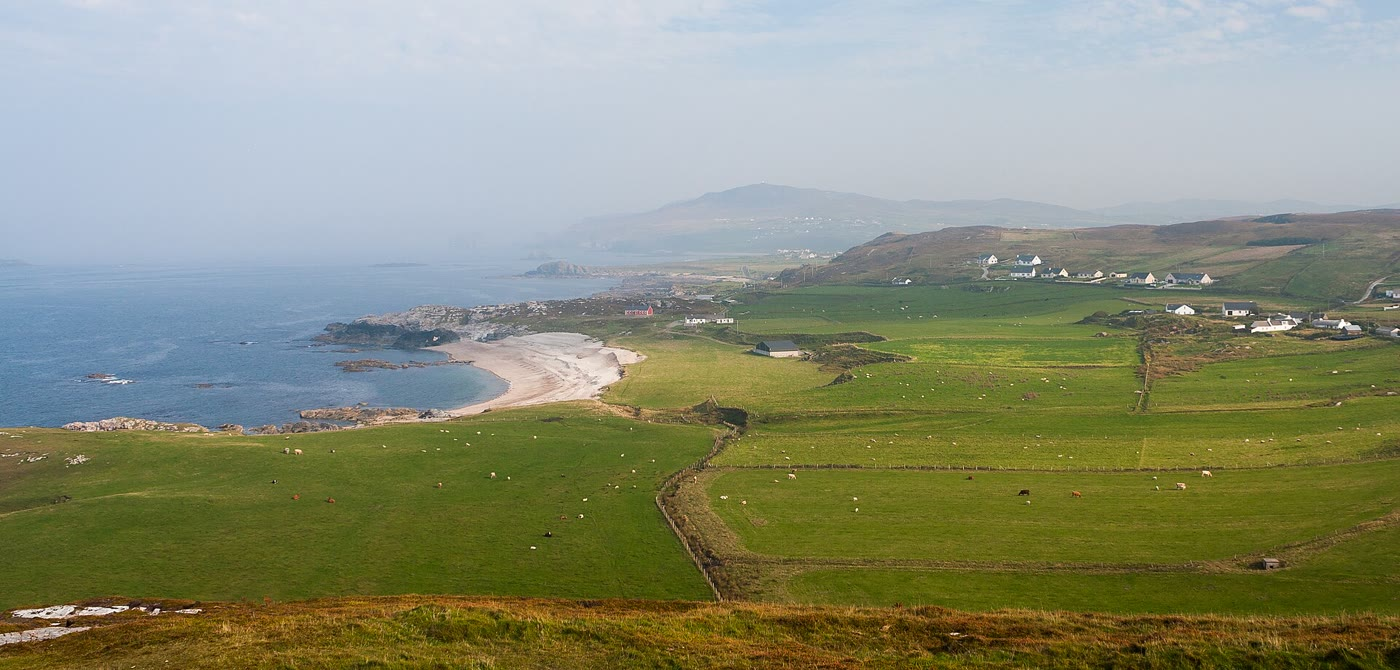
\includegraphics[width=\linewidth]{images/book5/b3-raised-beach-malin.jpg}

{\scriptsize الشواطئ المرتفعة في بالي هيلين، مالين هيد، شمال
أيرلندا: حواجز من الحصى لخطوط شواطئ قديمة رُفعت فوق البحر مع ارتفاع الأرض
بعد ذوبان غطائها الجليدي. الصورة: \mbox{\textdir TLT A.~F.~Borchert, CC BY-SA 4.0}.}
\end{minipage}
\end{inthefield}
% ledger: photo:b3-raised-beach

\section{الحمل الوشاحي الكامل وبنيته العميقة}

هل يتحرّك الوشاح حملًا في طبقة واحدة، أم في طبقتين، فوق الانقطاع
عند \qty{670}{km} وتحته؟ يُجيب التصوير المقطعي (انظر \cref{ch:b3:seismology-imaging})
جزئيًا عن ذلك: تتسطّح بعض اللوحات المندسّة فوق الانقطاع، بينما تغوص أخرى
عبره إلى الوشاح السفلي، فتعبر الكتلة منه، ولا تكون الطبقتان
معزولتين إحداهما عن الأخرى. يجعل ازدياد اللزوجة مع العمق الوشاح السفلي
يتدفّق ببطء أكبر، وتتباطأ اللوحات المندسّة وتتثخّن عند دخولها إليه.

عند قاع الوشاح، يُظهر التصوير المقطعي منطقتين واسعتين ذواتي سرعة منخفضة لموجات S
تحت أفريقيا وتحت المحيط الهادئ، وهما الأقاليم الكبيرة ذات السرعة المنخفضة للقصّ
\babelsublr{(LLSVPs)}. يُرجَّح أنّها متمايزة كيميائيًا عن الوشاح الذي يعلوها
وأكثف منه، فهي أكوام لا أعمدة حارّة. أمّا الأقاليم البركانية النارية الكبيرة
والكيمبرلايتات في المئات القليلة الأخيرة من ملايين السنين اندفعت في معظمها فوق
حوافّها، كأنّ الأعمدة صعدت من أطراف الأكوام، حيث تُجرف الطبقة الحدّية
الحارّة عند قاع الوشاح باتجاهها.
% ledger: st12:llsvp

\section{التمارين}

\begin{exercise}[$\star$]\label{exo:b3:mantle-convection:1}
احسب \omterm{def:b3:mantle-convection:rayleigh}{عدد رايلي} لطبقة من الوشاح العلوي سمكها \qty{670}{km} مع
$\rho = \qty{3500}{kg.m^{-3}}$، و$g = \qty{9.9}{m.s^{-2}}$، و$\alpha =
\qty{3e-5}{K^{-1}}$، و$\Delta T = \qty{1000}{K}$، و$\kappa =
\qty{e-6}{m^2.s^{-1}}$، و$\eta = \qty{5e20}{Pa.s}$. كم مرّة يتجاوز
\omterm{def:b3:mantle-convection:critical}{عدد رايلي الحرج}، بالنسبة إلى حدود انزلاق حرّ؟
\end{exercise}

\begin{exercise}[$\star$]\label{exo:b3:mantle-convection:2}
احسب \omterm{def:b3:mantle-convection:maxwell}{زمن ماكسويل} لوشاح لزوجته \qty{e21}{Pa.s} ومعامل
القصّ \qty{7.7e10}{Pa}، بالسنوات. هل يستجيب الوشاح مرنًا أم
لزجًا للمدّ الأرضي نصف اليومي، ولذوبان الغطاء الجليدي، ولغوص
لوح مندسّ؟
\end{exercise}

\begin{exercise}[$\star$]\label{exo:b3:mantle-convection:3}
مع $\eta = \qty{e21}{Pa.s}$، و$\rho = \qty{3300}{kg.m^{-3}}$، و$g =
\qty{9.8}{m.s^{-2}}$، احسب \omterm{def:b3:mantle-convection:relaxation-time}{زمن الارتخاء الأيزوستاتي} لنصف فضاء منتظم
لأحمال طول موجتها 1000 و\qty{3000}{km}. أيّهما يتعافى أسرع؟
\end{exercise}

\begin{exercise}[$\star$]\label{exo:b3:mantle-convection:4}
مع $g = \qty{9.8}{m.s^{-2}}$، و$\rho_m = \qty{3300}{kg.m^{-3}}$، و$\rho_w =
\qty{1030}{kg.m^{-3}}$، و$\alpha = \qty{3.1e-5}{K^{-1}}$، و$T_m - T_0 =
\qty{1450}{K}$، و$\kappa = \qty{0.8e-6}{m^2.s^{-1}}$، و\qty{1}{Myr} $=
\qty{3.156e13}{s}$، احسب \omterm{prop:b3:mantle-convection:ridge-push}{قوة دفع الظهرة} عند \qty{50}{Myr}. كم مرّة
تكون أصغر من شدّ لوح مندسّ قدره \qty{4.6e13}{N.m^{-1}}؟
\end{exercise}

\begin{exercise}[$\star\star$]\label{exo:b3:mantle-convection:5}
كتلة من الوشاح عرضها \qty{10}{km}، أسخن من محيطها بمقدار
\qty{300}{K}، تصعد بالسرعة $\rho g\alpha\Delta Td^2/\eta$ (خذ $\rho =
\qty{3300}{kg.m^{-3}}$، و$g = \qty{9.8}{m.s^{-2}}$، و$\alpha = \qty{3e-5}{K^{-1}}$،
$\eta = \qty{e21}{Pa.s}$، و$\kappa = \qty{e-6}{m^2.s^{-1}}$). (أ) احسب زمن صعودها عبر حجمها نفسه
وزمن انتشارها $d^2/\kappa$، وبيّن
أنّ نسبتهما هي \omterm{def:b3:mantle-convection:rayleigh}{عدد رايلي} لها. (ب) هل تصعد أولًا أم تبرد أولًا؟ (ج)
كم ينبغي أن يكون حجمها حتى يبلغ \omterm{def:b3:mantle-convection:rayleigh}{عدد رايلي} لها 657.5؟
\end{exercise}

\begin{exercise}[$\star\star$]\label{exo:b3:mantle-convection:6}
لطبقة عمقها \qty{2891}{km} عند $\mathrm{Ra} = \num{e7}$، مع $\kappa =
\qty{e-6}{m^2.s^{-1}}$، و$k = \qty{3.1}{W.m^{-1}.K^{-1}}$، و$\Delta T =
\qty{1450}{K}$، و$\mathrm{Ra}_c = 657.5$، احسب سمك الطبقة الحدّية،
\omterm{def:b3:mantle-convection:nusselt}{وعدد نوسلت}، ومقياس السرعة بوحدة \unit{cm/yr}، وتدفّق الحرارة
التدفق الحراري.
\end{exercise}

\begin{exercise}[$\star\star$]\label{exo:b3:mantle-convection:7}
لدينا انتفاخ افتراضي للبقعة الساخنة مساحة مقطعه العرضي \qty{8e8}{m^2} عبر
المسار، والصفيحة فوقه تتحرّك بسرعة \qty{9}{cm/yr}. مع $\rho_m - \rho_w =
\qty{2270}{kg.m^{-3}}$، احسب دفق طفوه، ودفق حرارته مع $c_p =
\qty{1170}{J.kg^{-1}.K^{-1}}$ و$\alpha = \qty{3.1e-5}{K^{-1}}$. ما الكسر
الذي يمثّله من \qty{46.7}{TW} للأرض؟
\end{exercise}

\begin{exercise}[$\star\star$]\label{exo:b3:mantle-convection:8}
رأس عمود نصف قطره \qty{400}{km}، أخفّ من الوشاح بمقدار
\qty{30}{kg.m^{-3}}، يصعد عبر وشاح لزوجته \qty{e21}{Pa.s}. باستخدام
قانون ستوكس، احسب سرعته بوحدة \unit{m/yr}، والزمن الذي يستغرقه لصعود
\qty{2000}{km}.
\end{exercise}

\begin{exercise}[$\star\star$]\label{exo:b3:mantle-convection:9}
انخفضت منطقة بمقدار \qty{300}{m} عندما ذاب جليدها، قبل \qty{10}{kyr}،
وتتعافى بثابت زمني $\tau = \qty{4.4}{kyr}$. احسب الانخفاض المتبقّي اليوم
ومعدّل الرفع الحالي. قارن بالرفع \qty{10.3}{mm/yr} المقيس قرب
أوميو.
\end{exercise}

\begin{exercise}[$\star\star\star$]\label{exo:b3:mantle-convection:10}
(أ) من تعبير $F_{rp}$ في برهان
\cref{prop:b3:mantle-convection:ridge-push}، بيّن أنّ الحد الأول،
$\tfrac12(\rho_m - \rho_w)gw^2$، هو الحد الثاني داخل القوس. (ب) بيّن أنّ
$\int_0^\infty x\operatorname{erfc}x\,\mathrm dx = 1/4$، بالتكامل بالتجزئة.
(ج) باستخدام قيم التمرين 4، احسب الحدّين عند \qty{100}{Myr}.
\end{exercise}

\begin{exercise}[$\star\star\star$]\label{exo:b3:mantle-convection:11}
بيّن أنّ $f(k) = (\pi^2 + k^2)^3/k^2$ يبلغ أصغر قيمة له عند $k = \pi/\sqrt2$، حيث
يساوي $27\pi^4/4$. استنتج عرض زوج من خلايا الحمل عند البدء،
بوحدات $d$، وعرض خلية واحدة.
\end{exercise}

\begin{exercise}[$\star\star\star$]\label{exo:b3:mantle-convection:12}
صفيحة طولها \qty{6000}{km} تتحرّك بسرعة \qty{6}{cm/yr} فوق طبقة من الوشاح
سمكها \qty{150}{km}، لزوجتها \qty{e20}{Pa.s}، وقاعدتها ساكنة. (أ)
احسب \omterm{def:b3:mantle-convection:basal-drag}{السحب القاعدي} بوحدة \unit{MPa} وقوة السحب لكل وحدة طول من الصفيحة.
(ب) قارنها بدفع ظهرة قدره \qty{3.8e12}{N.m^{-1}} وشدّ لوح مندسّ قدره
\qty{4.6e13}{N.m^{-1}}. (ج) إذا وصل عُشر شدّ اللوح المندس إلى الصفيحة،
فبأيّ سرعة يتعادل السحب مع قوى الدفع؟
\end{exercise}

\section{مسألة: ارتداد بحيرة أردو}

\begin{problem}[{مسألة نهاية الأسبوع --- ارتداد حوض بحيرة متخيَّلة،
لزوجة الوشاح أسفله، والحمل الذي
تُتيحه تلك اللزوجة}]
\label{pb:b3:mantle-convection:1}
% values: calc/ch06.py; gia_relaxation.py, convection_scaling.py
بحيرة أردو، وهي بحيرة متخيَّلة، ملأت حوضًا عرضه \qty{250}{km}، حجزها
غطاءٌ جليدي، وبقيت بعمق \qty{300}{m} نحو خمسين ألف سنة. وقبل أربعة عشر
ألف سنة انهار السدّ الجليدي، وتصرّفت البحيرة في بضعة أسابيع. وأعلى
خط شاطئ لها، وكان أفقيًّا حين تكوّن، فهو الآن مائل؛ وخطوط الشاطئ المؤرَّخة
للبحيرات الصغيرة المتبقّية في الحوض تعطي رفع المركز منذ التصرّف، بالنسبة إلى الحافة،
التي بالكاد تحرّكت:

\smallskip
\begin{center}\small
\begin{tabular}{lcccccc}
\hline
الزمن منذ التصرّف \babelsublr{(\unit{kyr})} & 1 & 2 & 4 & 6 & 9 & 14\\
الرفع في المركز \babelsublr{(m)} & 11.5 & 21.6 & 38.0 & 50.5 & 64.0 & 77.2\\
\hline
\end{tabular}
\end{center}
\smallskip

ليكن $\rho_w = \qty{1000}{kg.m^{-3}}$، و$\rho_m = \qty{3300}{kg.m^{-3}}$، و$g =
\qty{9.8}{m.s^{-2}}$، و\qty{1}{yr} $= \qty{3.156e7}{s}$، ونعامل الوشاح بوصفه
نصف فضاء لزج متجانس.

\medskip\noindent\textbf{الجزء الأول --- الحمولة.}
\begin{enumerate}
  \item احسب ضغط البحيرة على قاعها.
  \item احسب هبوط القاع عند التوازن الأيزوستاتي، وبيّن
        لماذا تظهر فيه كثافة الوشاح لا كثافة القشرة.
  \item عامِل البحيرة قرصًا واحسب كتلة مائها.
  \item فسّر لماذا أعلى خط شاطئ مائل الآن، واحسب
        متوسط ميله من الحافة إلى المركز، بالمتر لكل كيلومتر.
  \item عامِل الهبوط توافقيًّا واحدًا نصفه المنخفض، من
        $-\lambda/4$ إلى $\lambda/4$، يغطي البحيرة. أعطِ $\lambda$ و$k =
        2\pi/\lambda$.
  \item عند أيّ عمق يتناقص التدفق تحت حمولة كهذه بالمعامل
        $e$؟
\end{enumerate}

\medskip\noindent\textbf{الجزء الثاني --- زمن الارتخاء.}
\begin{enumerate}[resume]
  \item بافتراض أنّ البحيرة بلغت التوازن، احسب الهبوط المتبقّي
        عند كلّ تاريخ في الجدول.
  \item بيّن أنّه إذا تناقص الهبوط أُسّيًّا، فإنّ لوغاريتمه يتناقص
        خطيًّا مع الزمن.
  \item احسب $\tau$ من التاريخين 1 و\qty{14}{kyr}.
  \item تنبّأ بالرفع عند \qty{6}{kyr} باستعمال $\tau$ المحسوبة، وقارنه مع
        الجدول.
  \item احسب الهبوط المتبقّي اليوم ومعدّل الرفع الحالي للمركز،
        بوحدة \unit{mm/yr}.
  \item كم من الرفع ما زال باقيًا؟
  \item بعد كم سنة أخرى سينخفض معدّل الرفع دون
        \qty{0.5}{mm/yr}؟
\end{enumerate}

\medskip\noindent\textbf{الجزء الثالث --- اللزوجة.}
\begin{enumerate}[resume]
  \item احسب لزوجة نصف الفضاء من $\tau$.
  \item قارنها بلزوجات الوشاح العلوي المحصورة بين \num{3.4e20}
        و\qty{1e21}{Pa.s} التي وُجدت أسفل فينوسكانديا.
        أيّ جزء من الوشاح يسبره ارتداد بحيرة أردو؟
  \item بتلك اللزوجة، احسب زمن الارتخاء لحمولة
        \qty{3000}{km} طول موجتها. لماذا يرتخي غطاء جليدي حقيقي بهذا الحجم
        أبطأ من هذا؟
  \item ماذا يفعل الغلاف الصخري المرن، الذي أُهمل هنا، في ارتداد
        حمولة لا يتجاوز عرضها \qty{250}{km}؟
  \item احسب \omterm{def:b3:mantle-convection:maxwell}{زمن ماكسويل} للوشاح باستخدام $\mu = \qty{7.7e10}{Pa}$،
        وبيّن إن كان النموذج اللزج مبرَّرًا.
  \item تحقّق من الفرضية في السؤال 7: ما كسر هبوط التوازن الذي بلغته
        خلال بقاء البحيرة؟
  \item بمقدار كم سيتغيّر $\log_{10}\eta$ لو أُخذ $\lambda$ يساوي
        \qty{250}{km}؟
\end{enumerate}

\medskip\noindent\textbf{الجزء الرابع --- الحمل.} ليكن طبقة من الوشاح العلوي
عمقها \qty{670}{km} وكثافتها $\rho = \qty{3700}{kg.m^{-3}}$، و$g =
\qty{9.9}{m.s^{-2}}$، و$\alpha = \qty{3.1e-5}{K^{-1}}$، و$\Delta T =
\qty{1450}{K}$، و$\kappa = \qty{e-6}{m^2.s^{-1}}$، و$k = \qty{3.1}{W.m^{-1}.K^{-1}}$
واللزوجة الواردة في الجزء الثالث.
\begin{enumerate}[resume]
  \item احسب \omterm{def:b3:mantle-convection:rayleigh}{عدد رايلي} للطبقة.
  \item كم مرّةً يتجاوز الحدّ الحرج ($\mathrm{Ra}_c = 657.5$)؟
  \item احسب سمك الطبقة الحدّية \omterm{def:b3:mantle-convection:nusselt}{وعدد نوسلت}.
  \item احسب مقياس السرعة بوحدة \unit{cm/yr}، وقارنه بسرعات الصفائح
        التي تتراوح من 1 إلى \qty{7.5}{cm/yr}.
  \item احسب التدفق الحراري، وأعطِ سببين يفسّران قصوره عن
        المتوسط الأرضي البالغ \qty{92}{mW.m^{-2}}.
  \item أعطِ \omterm{def:b3:mantle-convection:gia}{لزوجة الوشاح} العلوي أسفل بحيرة أردو بوصفها $\log_{10}$ لقيمة
        $\eta$ بوحدة \unit{Pa.s}.
\end{enumerate}
\end{problem}
